\documentclass[11pt,a4paper,fontset=fandol]{ctexart}

% ====== 版面 ======
\usepackage{geometry}
\geometry{a4paper, left=2.2cm, right=2.2cm, top=2.2cm, bottom=2.2cm, headheight=14pt}
\usepackage{setspace}
\linespread{1.05}
\usepackage{indentfirst}
\setlength{\parindent}{2em}
\emergencystretch=2em

% ====== 颜色 ======
\usepackage{xcolor}
\definecolor{themecolor}{RGB}{40,90,140}
\definecolor{codebg}{RGB}{248,248,245}

% ====== 图、表、数学 ======
\usepackage{graphicx}
\graphicspath{{results/}}
\usepackage{amsmath}
\usepackage{booktabs}
\usepackage{caption}
\captionsetup{font=small,labelfont={bf,color=themecolor}}
\usepackage{subcaption}
\usepackage{float}
\usepackage{array}
\usepackage{makecell}
\usepackage{verbatim}

% ====== 链接 ======
\usepackage{hyperref}
\hypersetup{
  colorlinks=true,
  linkcolor=themecolor,
  citecolor=themecolor,
  urlcolor=themecolor!70!black,
}

% ====== 章节样式：主题色 + 横线分割 ======
\usepackage{titlesec}
\titleformat{\section}
  {\color{themecolor}\bfseries\fontsize{13}{16}\selectfont}
  {\thesection}{0.6em}{}
\titlespacing*{\section}{0pt}{0.9em}{0.35em}

\titleformat{\subsection}
  {\color{themecolor!85!black}\bfseries\fontsize{11.5}{14}\selectfont}
  {\thesubsection}{0.6em}{}
\titlespacing*{\subsection}{0pt}{0.55em}{0.15em}

% ====== 页眉页脚 ======
\usepackage{fancyhdr}
\pagestyle{fancy}
\fancyhf{}
\renewcommand{\headrulewidth}{0.4pt}
\lhead{\small\color{black!55} 路径规划实验报告}
\rhead{\small\color{black!55} 人工智能 2302}
\cfoot{\small\color{black!55}\thepage}

\fancypagestyle{plain}{
  \fancyhf{}
  \renewcommand{\headrulewidth}{0pt}
  \cfoot{\small\color{black!55}\thepage}
}

% ====== 代码块加浅色边框 ======
\usepackage{mdframed}
\BeforeBeginEnvironment{verbatim}{
  \begin{mdframed}[
    backgroundcolor=codebg,
    linecolor=themecolor!30,
    linewidth=0.5pt,
    innerleftmargin=10pt,
    innerrightmargin=8pt,
    innertopmargin=6pt,
    innerbottommargin=4pt,
    skipabove=8pt,
    skipbelow=8pt,
    roundcorner=2pt,
  ]
}
\AfterEndEnvironment{verbatim}{\end{mdframed}}

\setCJKmonofont{Arial Unicode MS}

% ====== 标题页信息 ======
\title{\bfseries 路径规划实验报告}
\author{人工智能2302 \quad 蒋梓轩\\
人工智能2302 \quad 汪翌秦\\
人工智能2302 \quad 孙靖淞}
\date{2026 年 5 月 29 日}

\begin{document}

\maketitle

\section{实验目的}

本次实验在实验 3 已构建的静态栅格地图和实验 4 的 AMCL 定位基础上，进一步添加 ROS 导航栈中的 \verb|move_base| 功能包，实现移动机器人从当前位置到目标点的自主路径规划、局部轨迹跟踪和实时避障。实验重点不是单纯让机器人走到目标点，而是理解 \verb|map_server|、AMCL、全局/局部代价地图、全局规划器、局部规划器以及底盘速度控制之间的数据流。

通过本次实验，需要掌握四个重点：第一，理解全局路径规划和局部路径规划在导航系统中的分工；第二，理解代价地图如何把静态地图、实时障碍物和膨胀层融合为路径搜索空间；第三，掌握 \verb|move_base| 节点与 AMCL、地图服务、传感器和底盘控制器之间的交互关系；第四，验证在 Gazebo 中增加未知障碍物后，局部代价地图能否实时更新并辅助机器人完成动态避障。

\section{实验原理}

移动机器人导航通常采用全局规划和局部规划协同工作的分层结构。全局规划器基于静态地图和全局代价地图，在 \verb|map| 坐标系下生成从当前位置到目标点的宏观路径；局部规划器则在 \verb|odom| 坐标系下结合实时激光雷达数据和局部代价地图，采样可行速度并输出 \verb|/cmd_vel|，使机器人尽量贴合全局路径前进，同时避开临时出现的障碍物。

\verb|move_base| 是 ROS 导航栈中的核心控制节点。它接收目标点后调用全局规划器生成路径，再调用局部规划器生成速度指令。若局部规划失败或路径被阻塞，\verb|move_base| 会重新规划，必要时触发清除代价地图、原地旋转等恢复行为。导航目标如果通过 RViz 工具栏的 2D Nav Goal 发布，则会被发送到 \verb|/move_base_simple/goal|；更完整的程序化导航任务则可以通过 \verb|move_base| Action 接口发送目标、接收反馈并在必要时取消任务。

代价地图将环境转化为 0 到 255 的栅格代价值。自由区域代价接近 0，障碍物区域为致命代价，障碍物周围由 \verb|inflation_layer| 生成膨胀区，表示机器人靠近障碍物时的碰撞风险。全局代价地图主要服务于宏观路径搜索，局部代价地图则维护机器人附近的滚动窗口，频率更高，能融合 \verb|/scan| 激光数据标记新增障碍物并清除已消失障碍物。

\begin{table}[H]
  \small
  \setlength{\tabcolsep}{3pt}
  \centering
  \caption{本实验中的关键配置文件与作用}
  \begin{tabular}{p{0.23\linewidth}p{0.27\linewidth}p{0.41\linewidth}}
    \toprule
    配置文件 & 关键参数 & 作用 \\
    \midrule
    \makecell[l]{\texttt{costmap\_common}\\\texttt{\_params.yaml}} & \makecell[l]{\texttt{robot\_radius}\\\texttt{obstacle\_range}\\\texttt{raytrace\_range}\\\texttt{inflation\_radius}\\\texttt{scan}} & 定义机器人安全半径、障碍物检测距离、射线清除距离、膨胀半径和激光雷达观测源。 \\
    \makecell[l]{\texttt{global\_costmap}\\\texttt{\_params.yaml}} & \makecell[l]{\texttt{global\_frame: map}\\\texttt{static\_map: true}} & 基于 \verb|map_server| 加载的静态地图维护全局代价地图，供全局规划器搜索。 \\
    \makecell[l]{\texttt{local\_costmap}\\\texttt{\_params.yaml}} & \makecell[l]{\texttt{global\_frame: odom}\\\texttt{rolling\_window: true}\\\texttt{3m x 3m}} & 维护机器人周围滚动窗口，融合实时激光信息进行局部避障。 \\
    \makecell[l]{\texttt{base\_local}\\\texttt{\_planner\_params.yaml}} & \makecell[l]{\texttt{max\_vel\_x}\\\texttt{xy\_goal\_tolerance}\\\texttt{sim\_time}\\\texttt{vx\_samples}} & 限制速度和加速度，设置局部轨迹采样与目标容差。 \\
    \bottomrule
  \end{tabular}
  \label{tab:configs}
\end{table}

\section{实验步骤与结果分析}

\subsection{导航功能包与配置文件整理}

按照指导书要求，在工作空间中加入 navigation 相关功能包，包括 \verb|move_base|、\verb|costmap_2d|、\verb|nav_core|、\verb|base_local_planner|、\verb|navfn|、\verb|clear_costmap_recovery|、\verb|rotate_recovery| 和 \verb|voxel_grid|。随后在 \verb|ebot_bringup/param| 中建立代价地图、局部规划器和 \verb|move_base| 配置文件，并在 launch 文件中统一加载。

\verb|nav02_path.launch| 负责启动 \verb|move_base| 并加载全局/局部代价地图、局部规划器和 \verb|move_base| 状态机参数；\verb|test_nav.launch| 先启动实验 4 中已经配置好的 \verb|test_amcl.launch|，以加载 \verb|map_server|、\verb|rf2o_laser_odometry| 和 AMCL，再启动 \verb|nav02_path.launch|，形成完整导航链路。

\begin{verbatim}
roslaunch ebot_bringup bringup.launch
roslaunch ebot_bringup test_nav.launch
\end{verbatim}

\subsection{静态地图加载、定位与目标发布}

运行 \verb|bringup.launch| 后，Gazebo 载入仿真场景与机器人模型，RViz 中显示 RobotModel、TF、LaserScan 和 Map。随后运行 \verb|test_nav.launch|，\verb|map_server| 发布 \verb|/map|，AMCL 根据静态地图和激光数据估计机器人在 \verb|map| 中的位姿，\verb|move_base| 等待目标点输入。

在 RViz 工具栏中使用 2D Nav Goal 选定目标位姿后，RViz 将目标点封装为 PoseStamped 消息发布到 \verb|/move_base_simple/goal|，\verb|move_base| 接收该目标并启动规划流程。图 \ref{fig:nav-goal} 显示了导航目标发布后的 RViz 状态。

\begin{figure}[H]
  \centering
  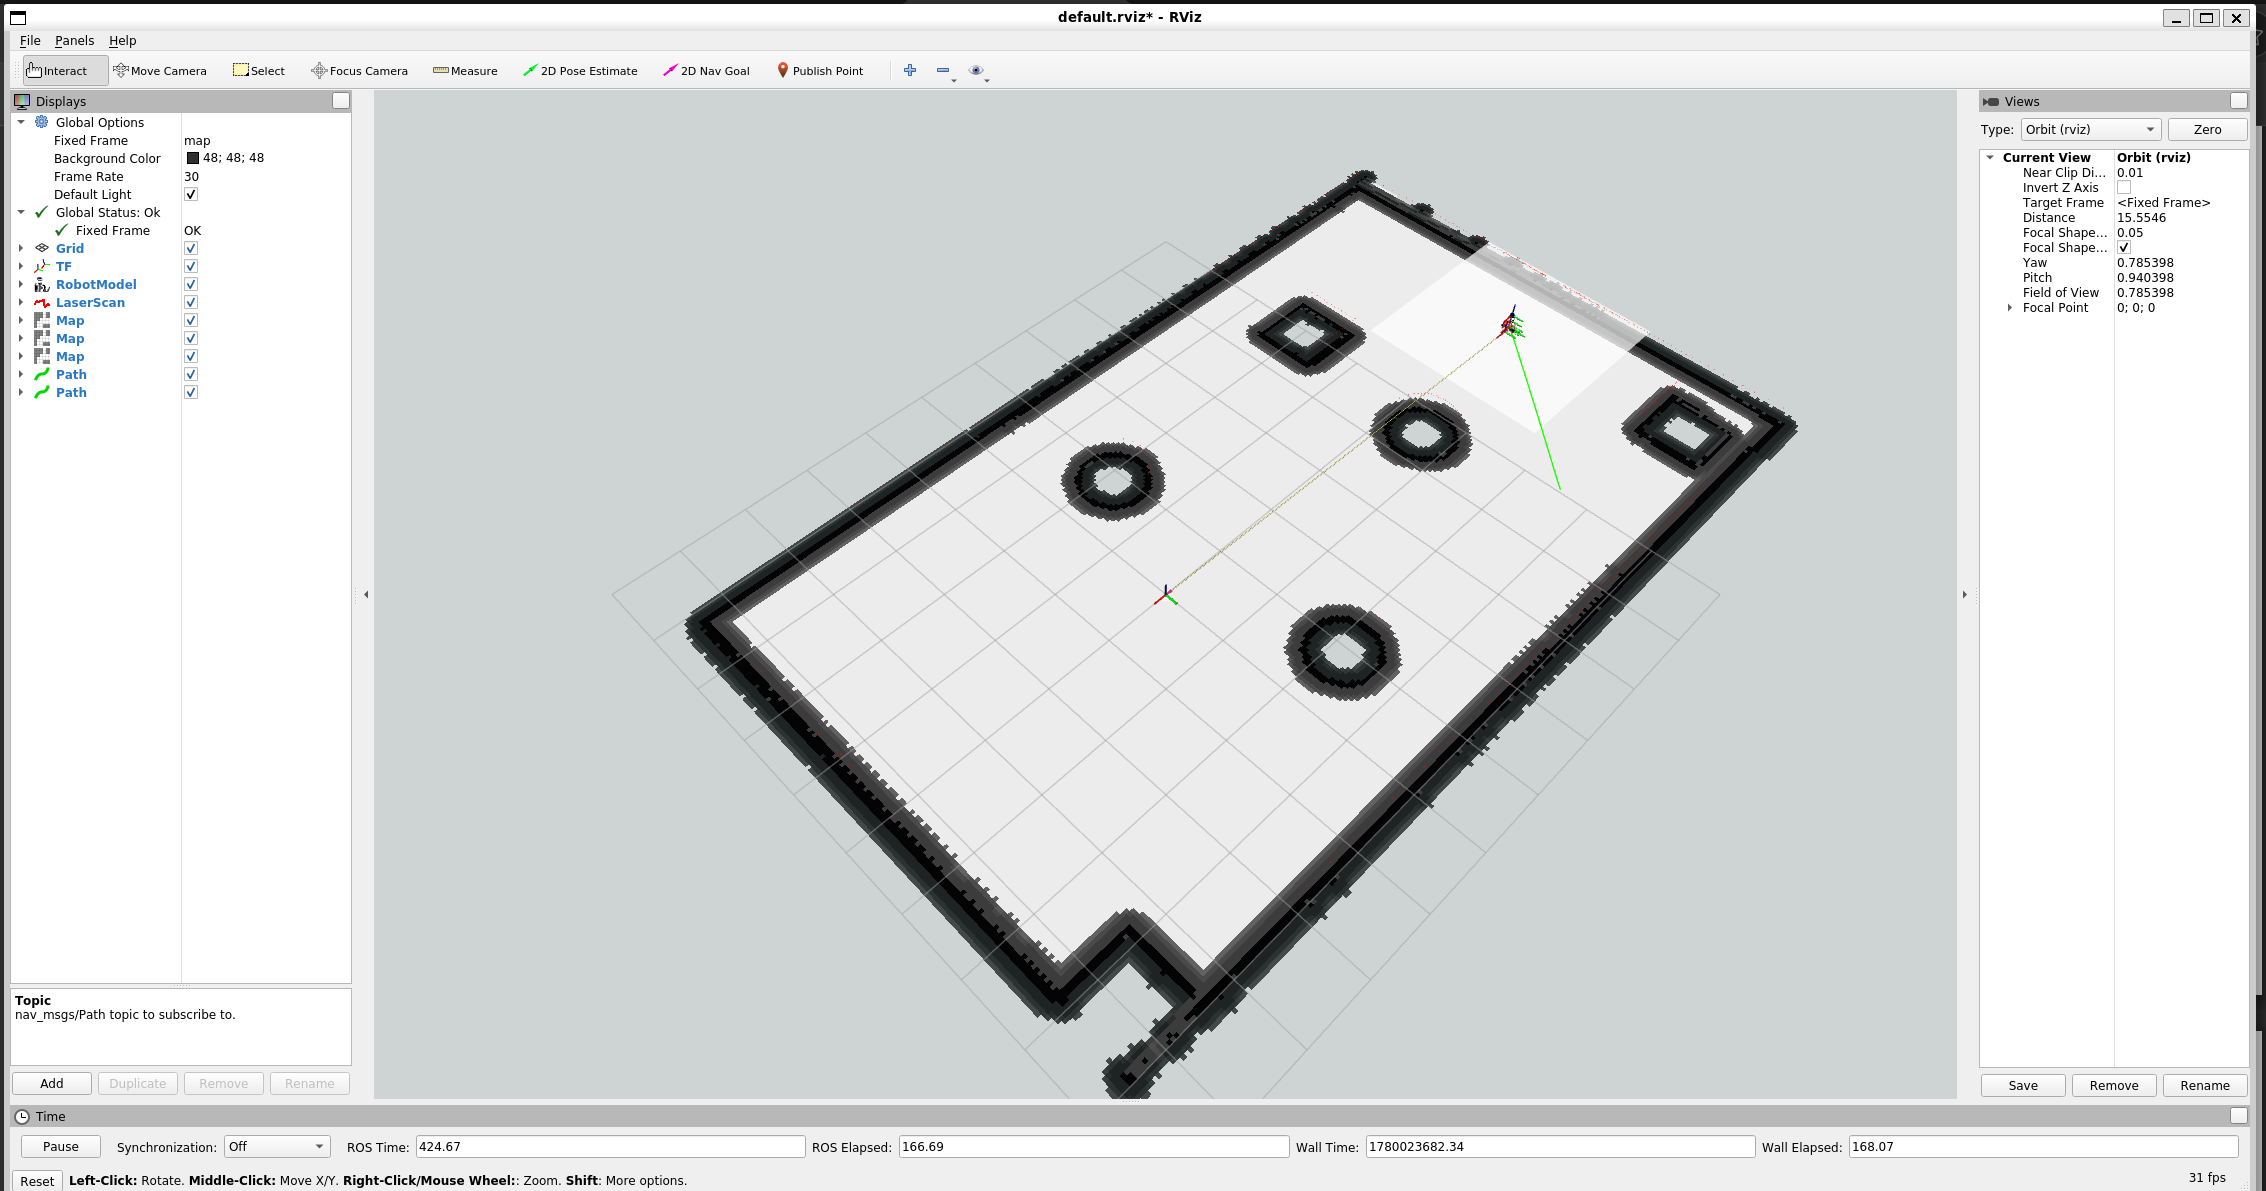
\includegraphics[width=0.92\linewidth]{nav_goal.png}
  \caption{在 RViz 中发布导航目标并显示机器人当前位姿。}
  \label{fig:nav-goal}
\end{figure}

\subsection{全局路径规划与局部路径跟踪}

目标点发布后，全局规划器基于静态地图和全局代价地图生成从当前位姿到目标点的路径，RViz 中以 Path 显示。机器人运动过程中，局部规划器持续接收全局路径和局部代价地图，在速度空间中采样候选轨迹，输出 \verb|/cmd_vel| 控制机器人前进和转向。

从实验截图可以看到，橙色路径沿着障碍物膨胀区外侧前进，机器人不会贴近圆柱或方块障碍物；局部路径在机器人周围短距离内更新，用于平滑跟踪全局路径。图 \ref{fig:path-plan} 中，左图为 RViz 中的路径规划显示，右图为 Gazebo 中机器人沿规划任务运动时的场景状态。

\begin{figure}[H]
  \centering
  \begin{subfigure}{0.49\linewidth}
    \centering
    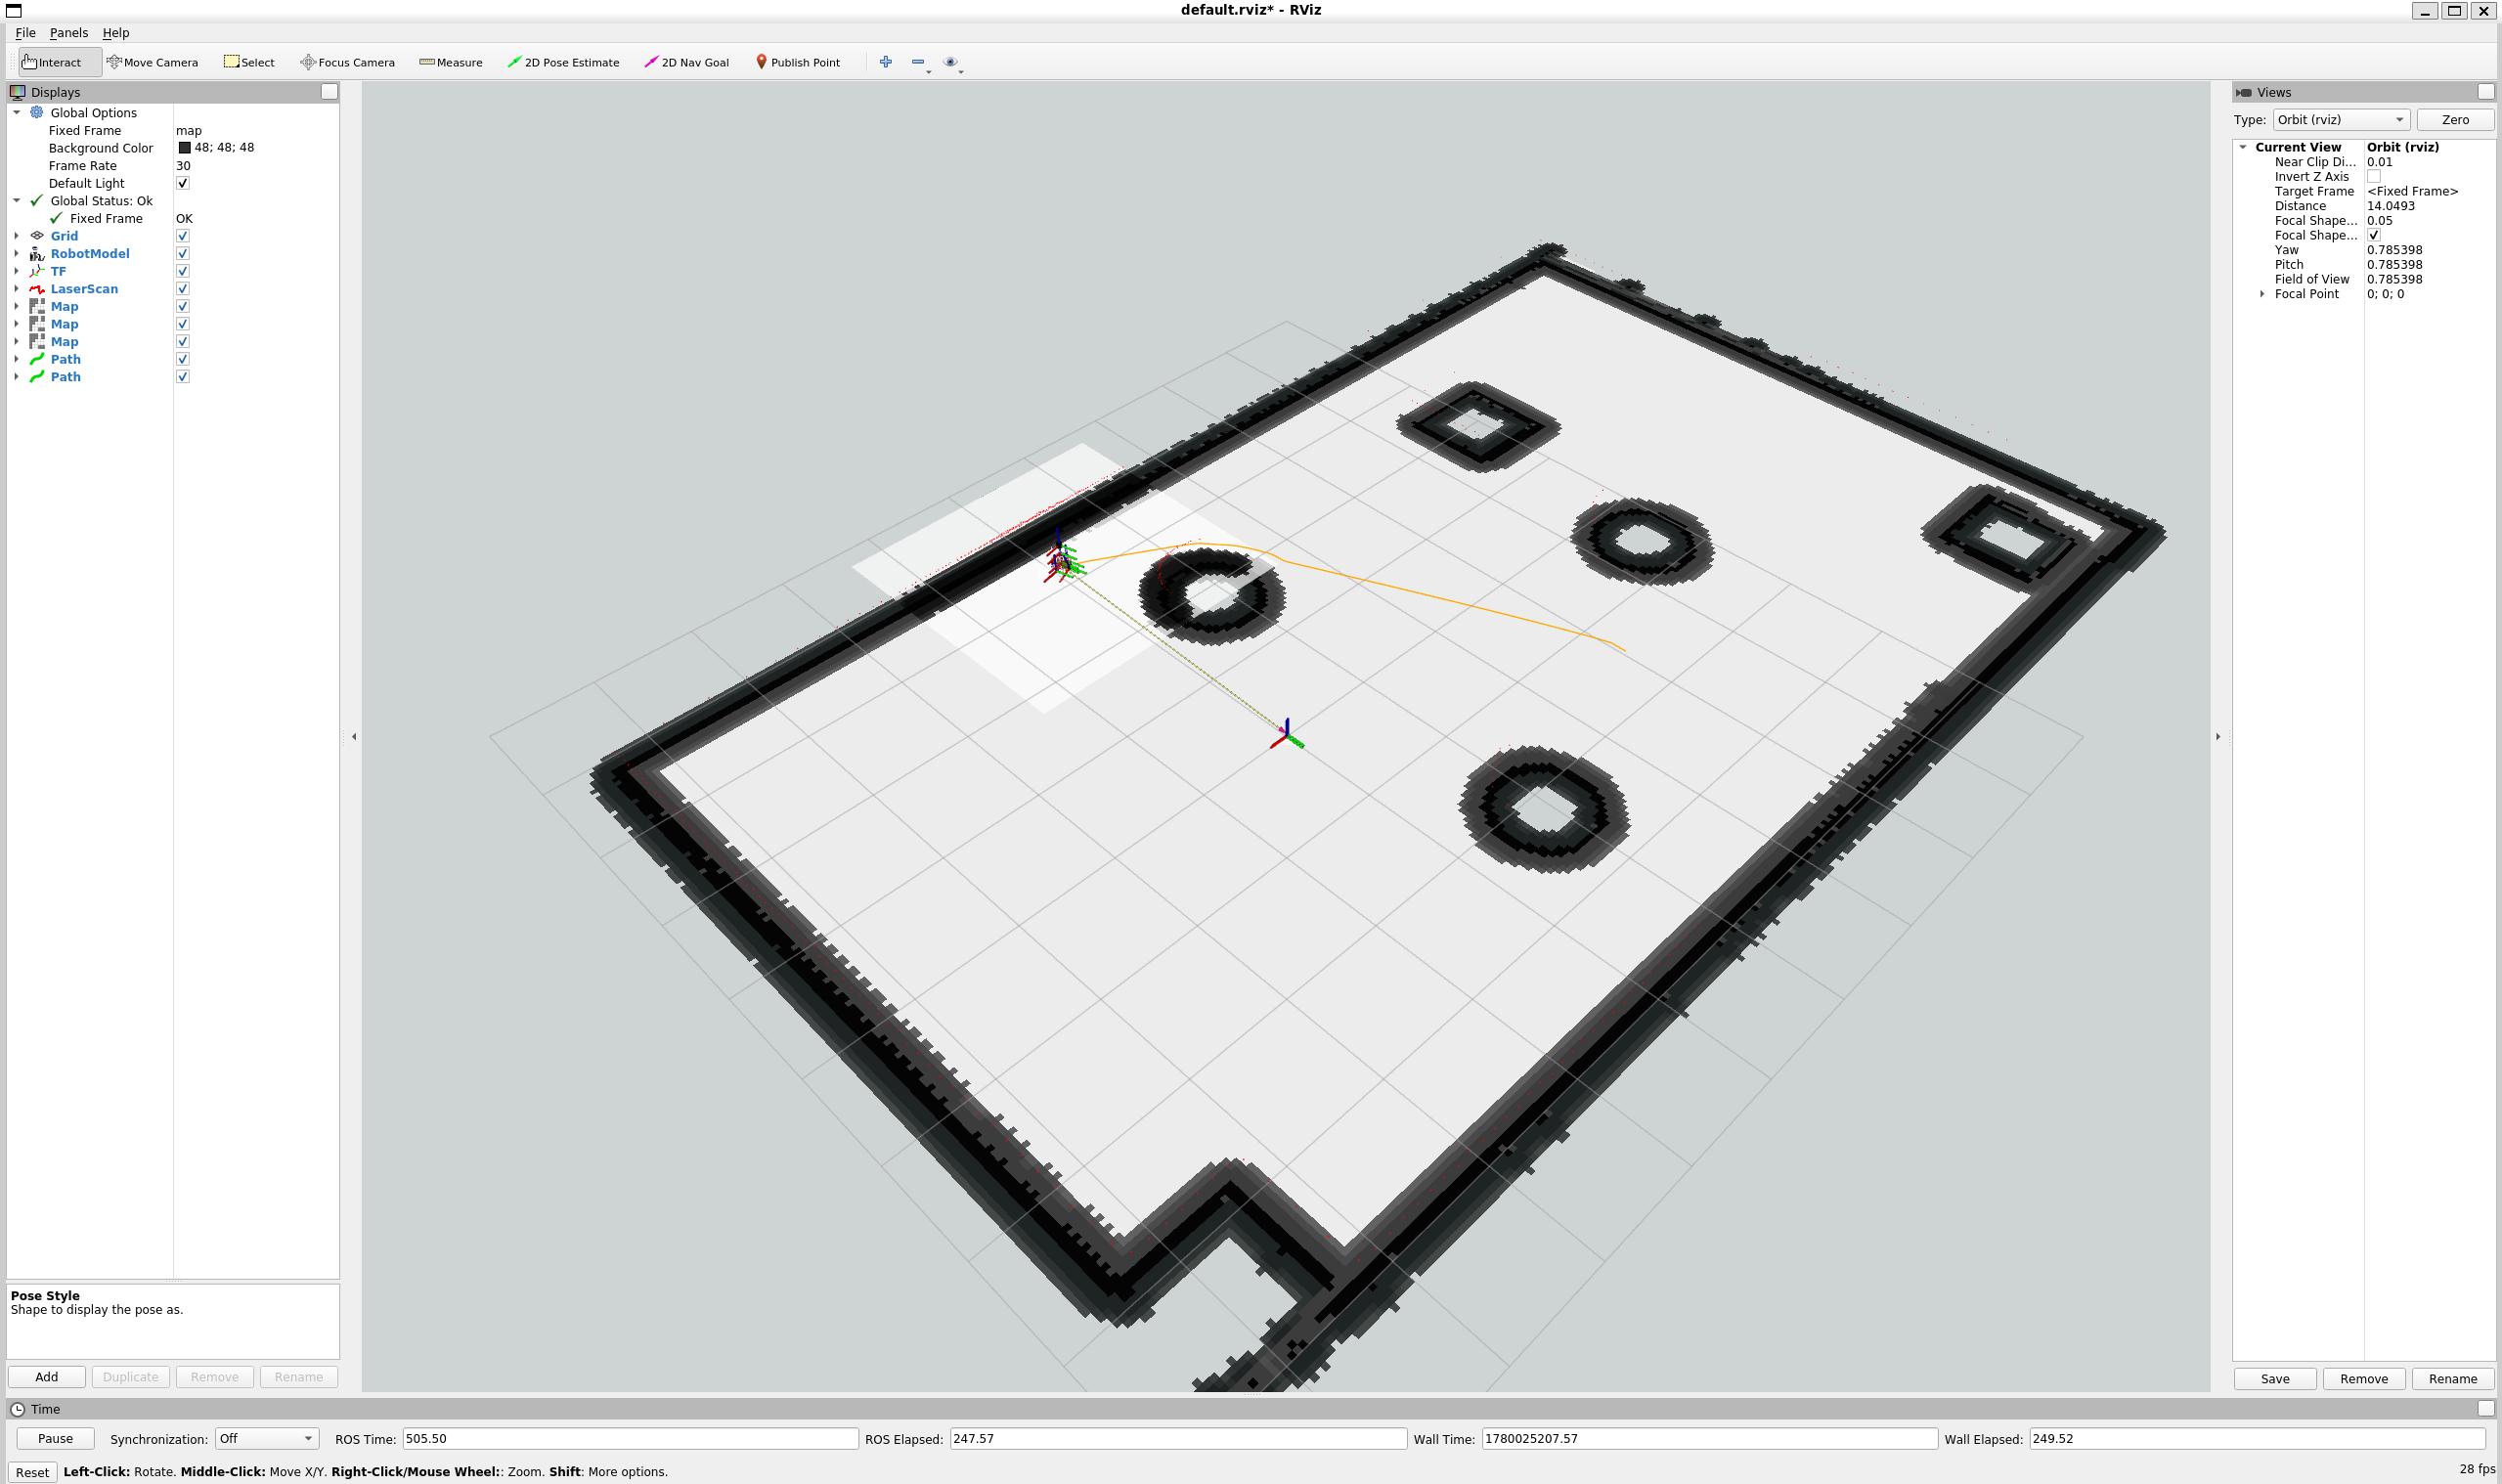
\includegraphics[width=\linewidth]{path_initial.png}
    \caption{全局路径和局部路径初始规划结果}
  \end{subfigure}
  \hfill
  \begin{subfigure}{0.49\linewidth}
    \centering
    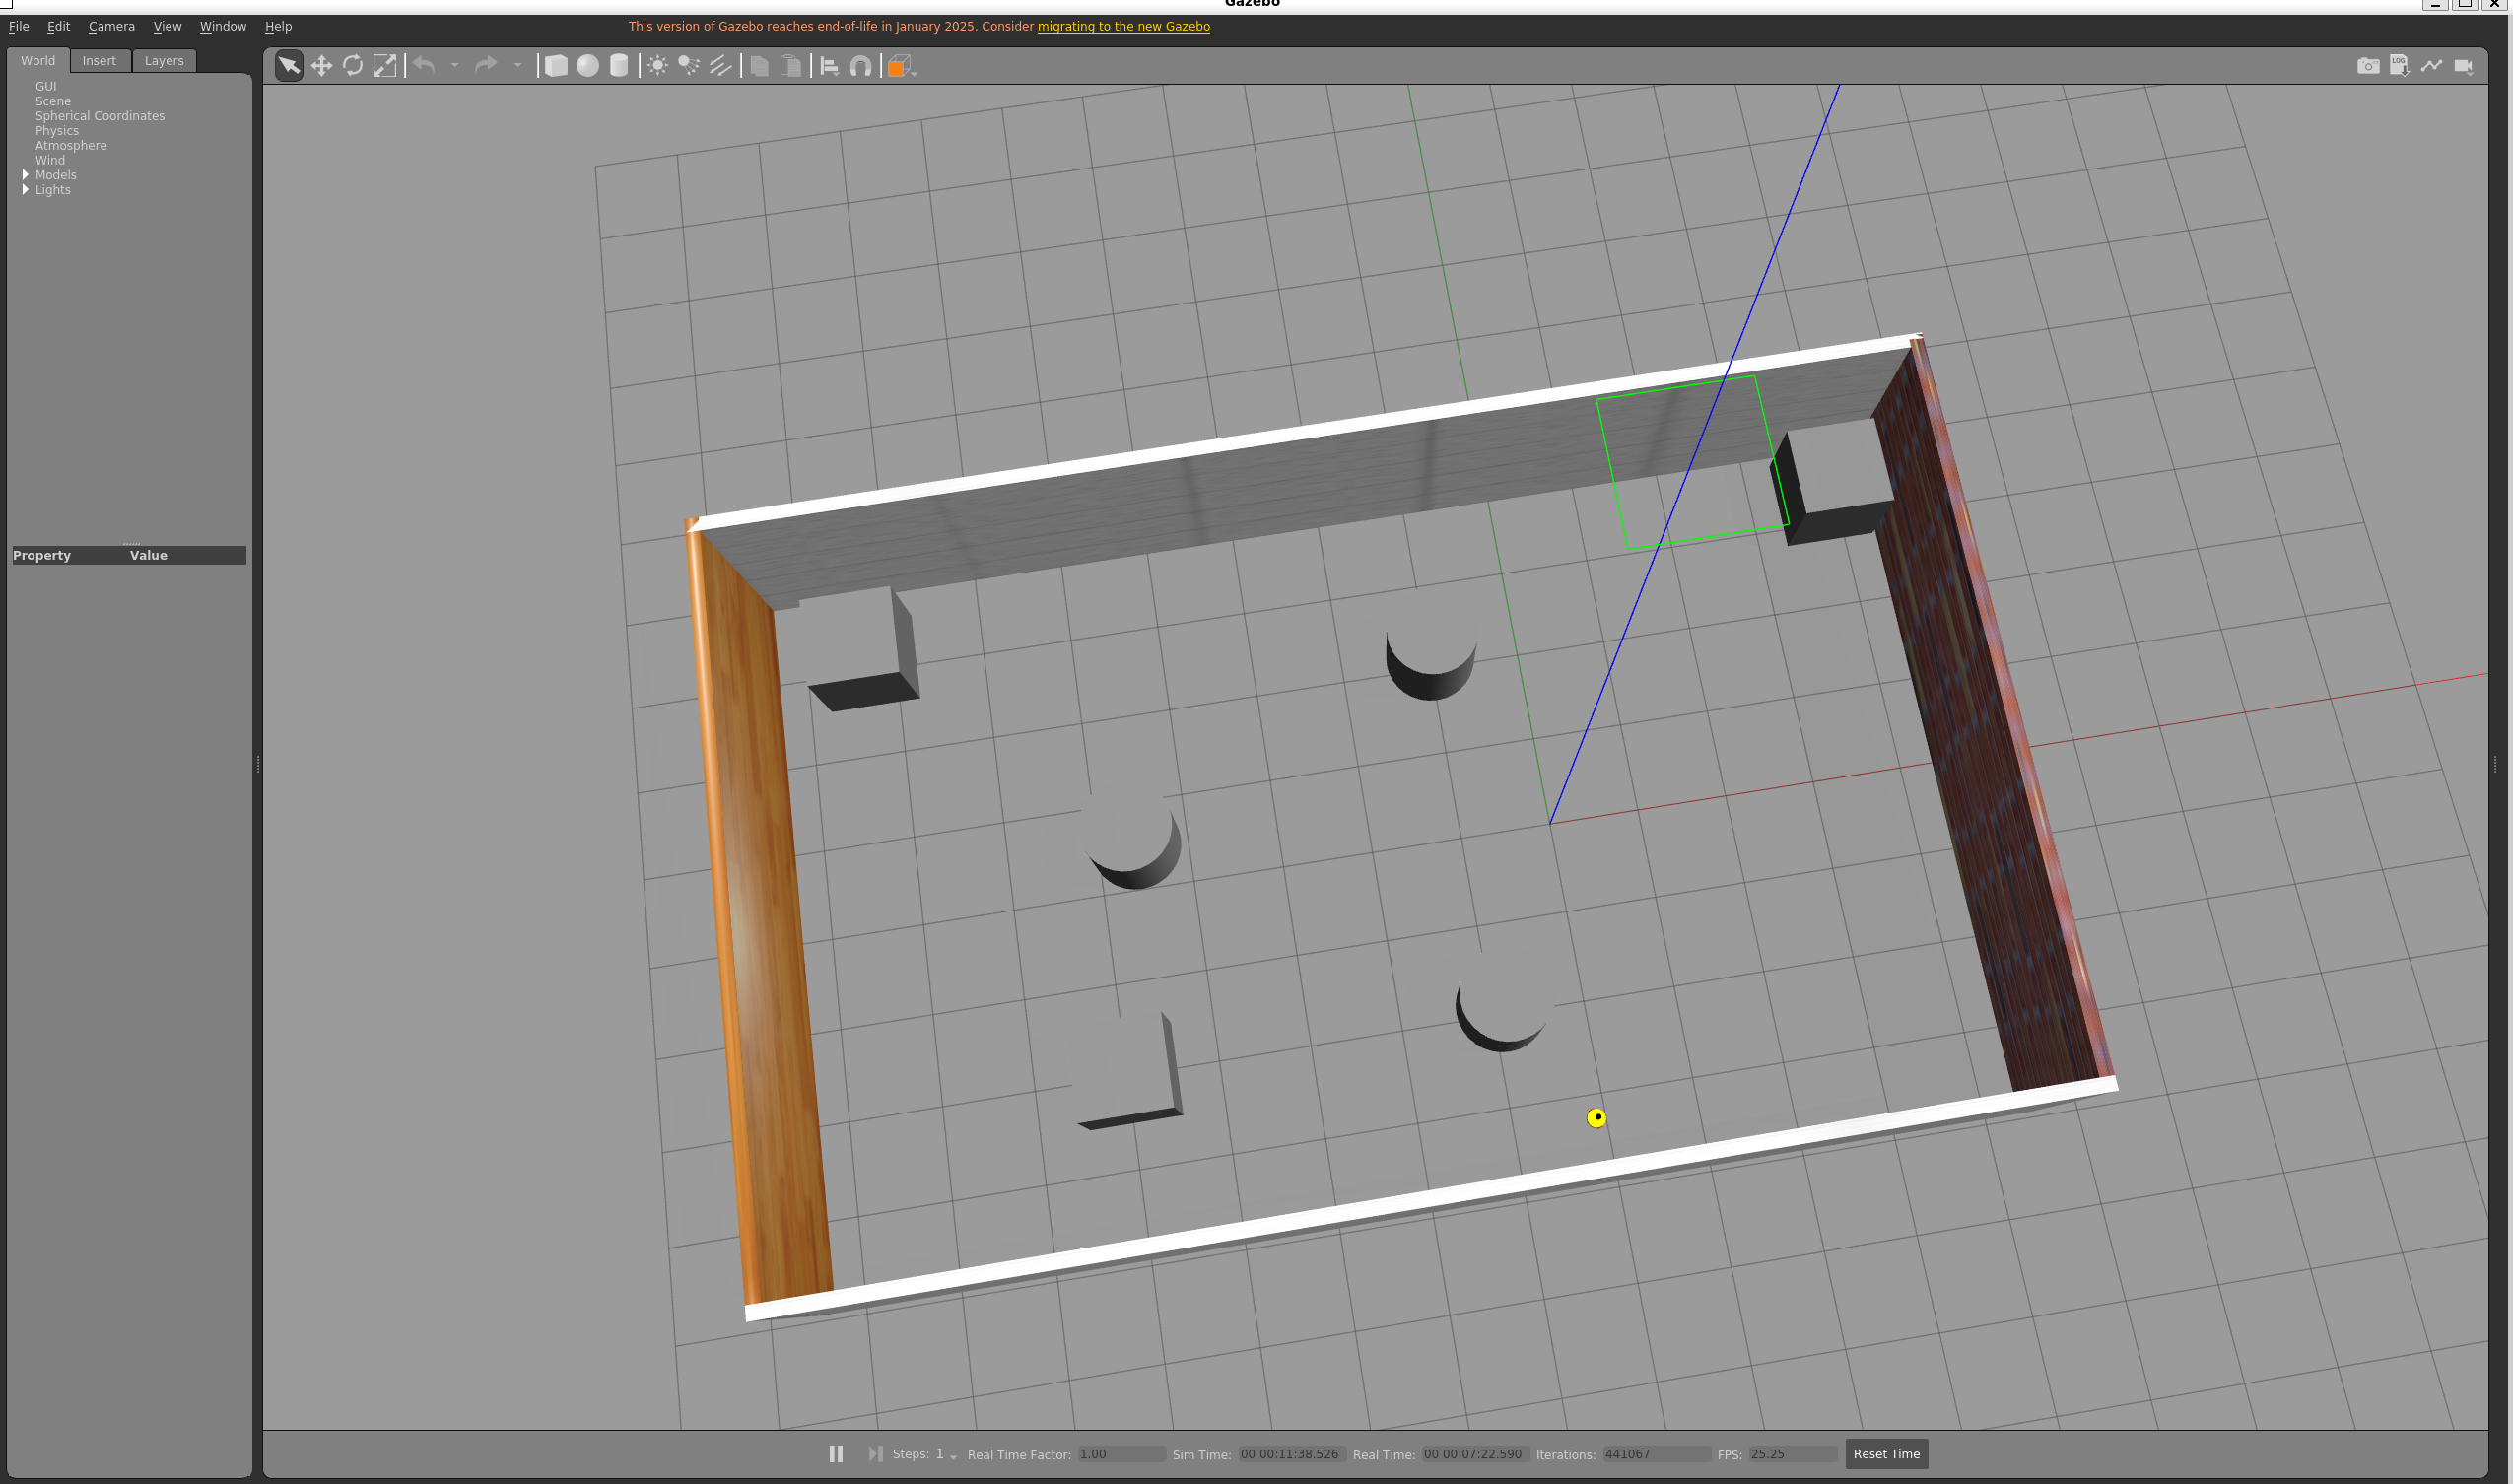
\includegraphics[width=\linewidth]{path_follow.png}
    \caption{Gazebo 中机器人沿规划任务运动}
  \end{subfigure}
  \caption{路径规划结果与 Gazebo 运动状态。}
  \label{fig:path-plan}
\end{figure}

\subsection{新增未知障碍物与局部代价地图更新}

为验证动态避障能力，在导航过程中向 Gazebo 场景中加入原始静态地图中不存在的障碍物。该障碍物不会立即改变 \verb|/map| 静态地图，但会被激光雷达检测到，并通过 \verb|obstacle_layer| 写入 \verb|local_costmap|。由于局部代价地图采用滚动窗口并以 10 Hz 更新，新增障碍物会在机器人附近快速变为致命障碍及膨胀区域。

图 \ref{fig:unknown-obstacle} 中，左图为 Gazebo 场景中加入的原静态地图未知障碍物，右图为 RViz 中对应的局部代价地图更新结果。右图中新增障碍物附近出现新的深色障碍区与灰色膨胀区，说明未知障碍物已经被实时感知并参与局部规划。局部规划器随后调整候选轨迹，从障碍物侧方绕行，避免继续沿原全局路径直接穿越障碍物。

\begin{figure}[H]
  \centering
  \begin{subfigure}{0.49\linewidth}
    \centering
    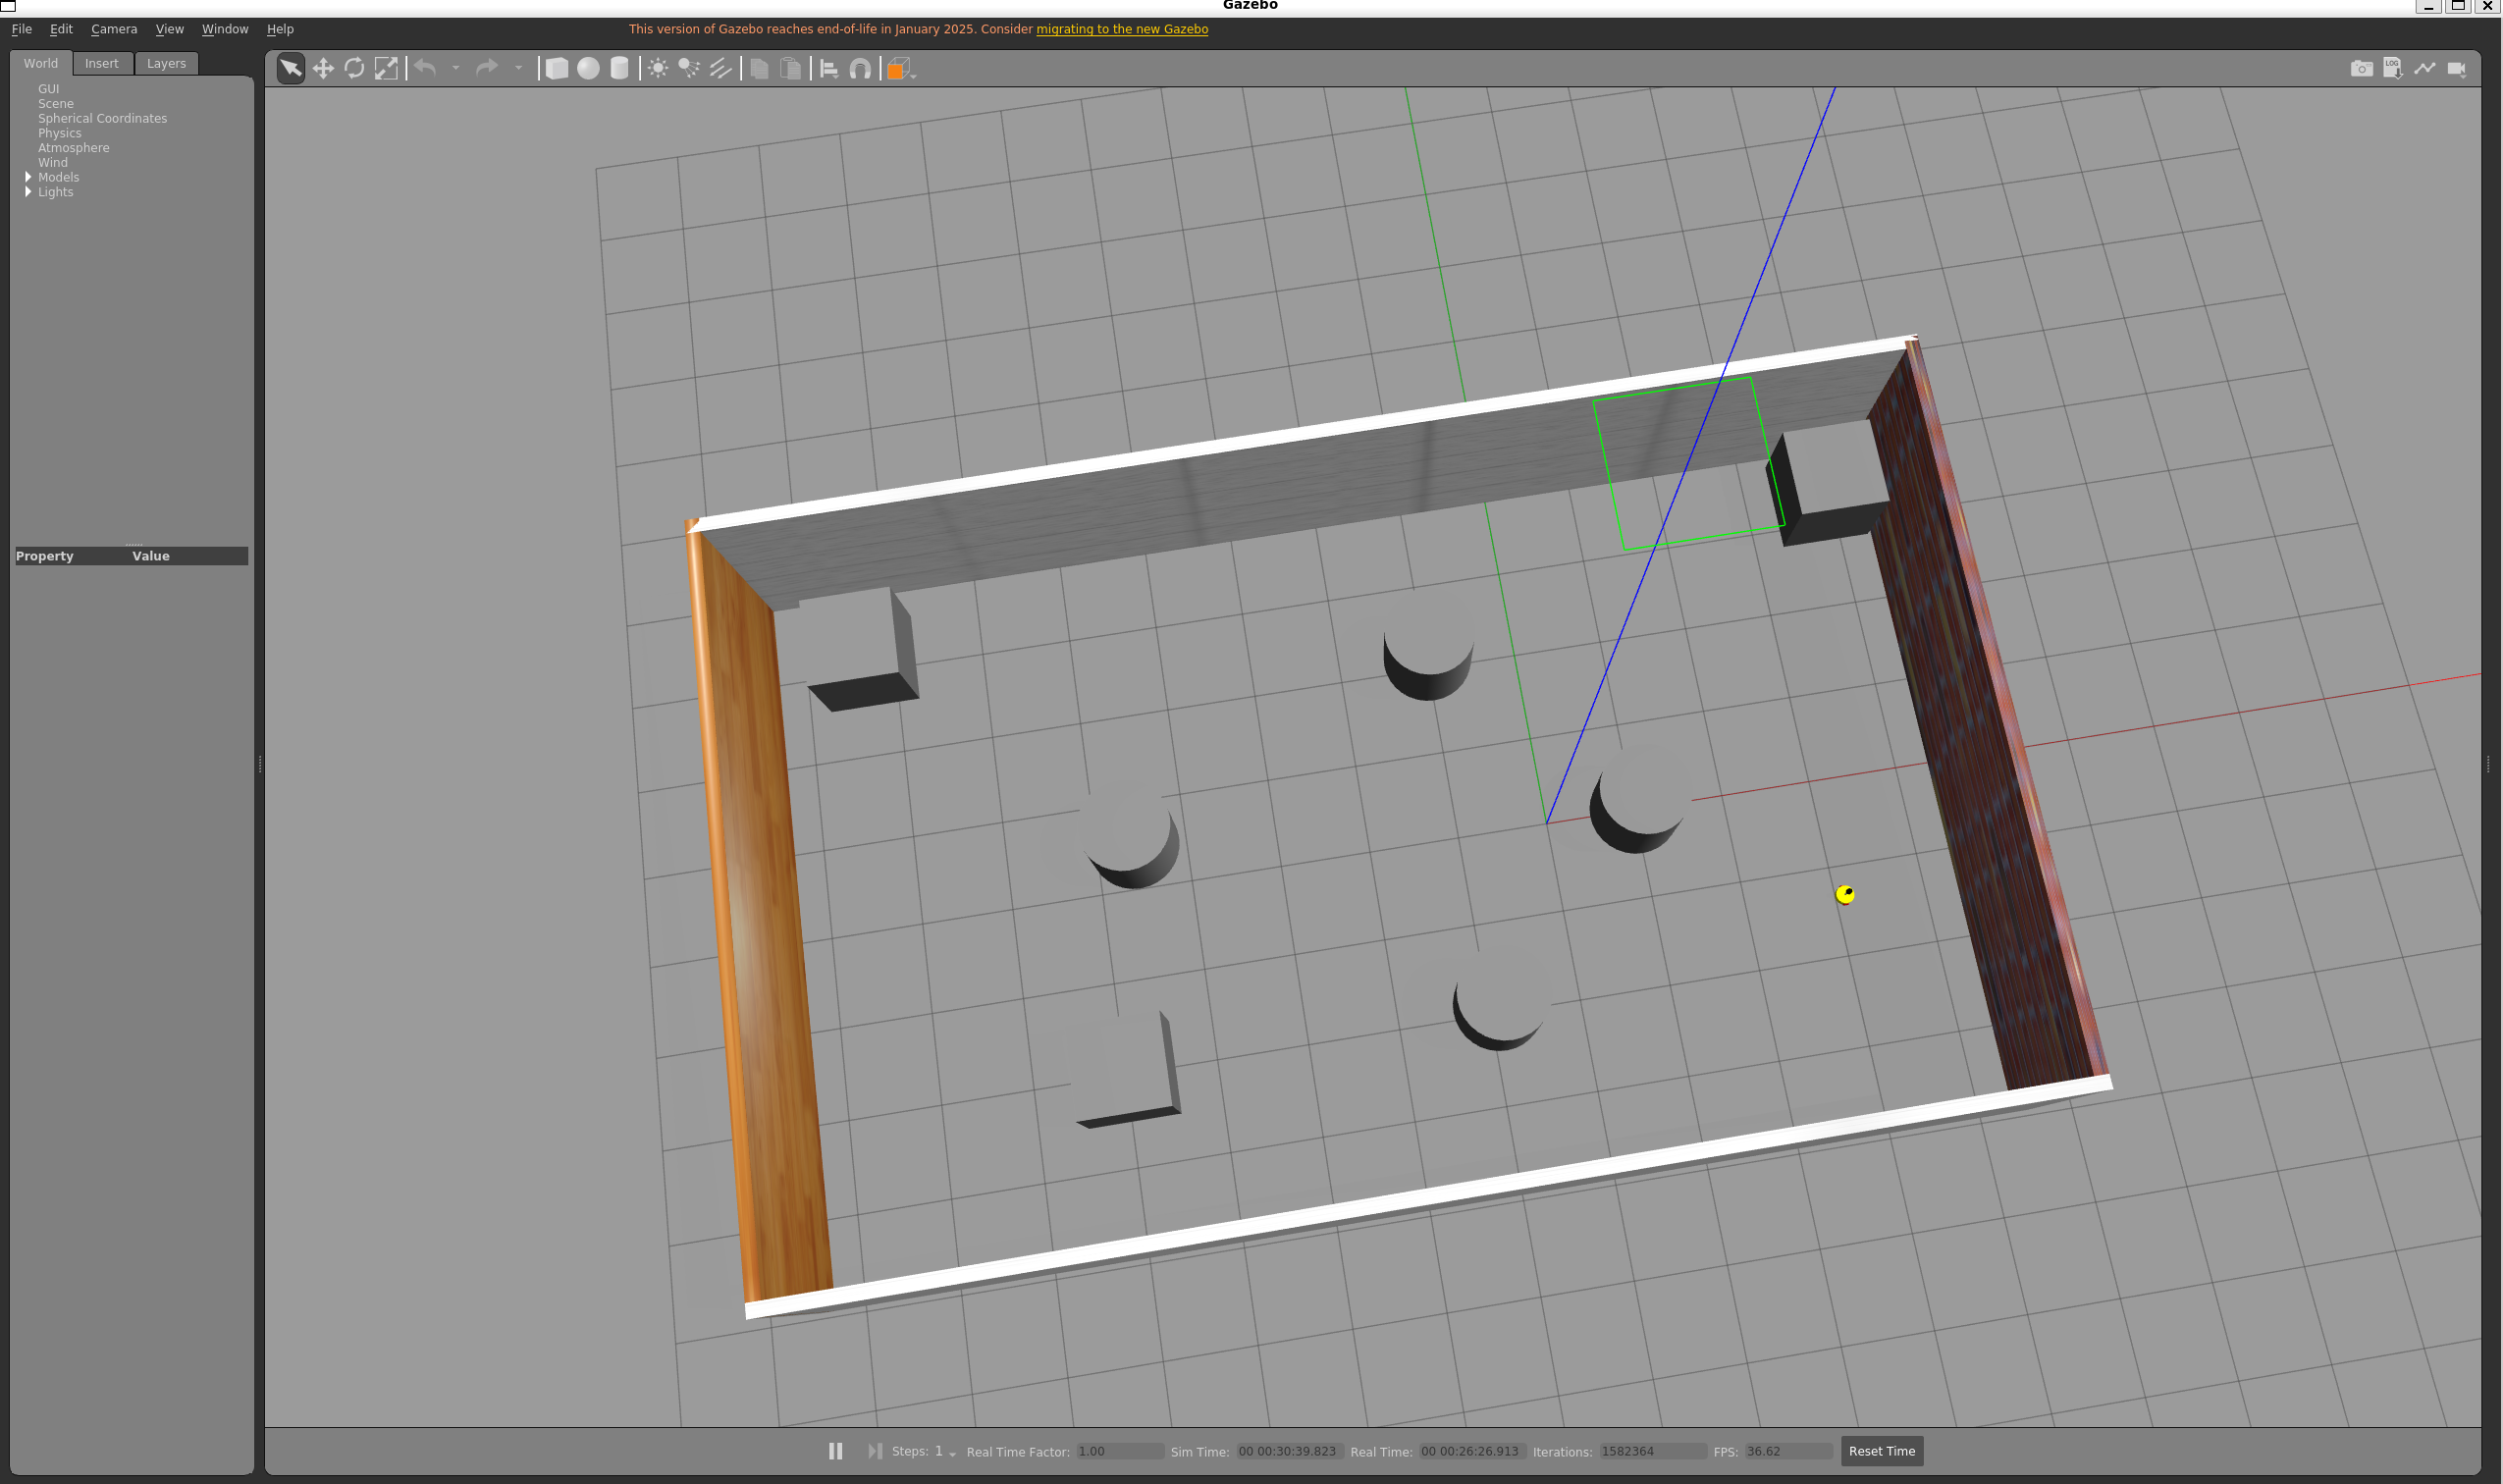
\includegraphics[width=\linewidth]{gazebo_unknown.png}
    \caption{Gazebo 中加入原静态地图未知的障碍物}
  \end{subfigure}
  \hfill
  \begin{subfigure}{0.49\linewidth}
    \centering
    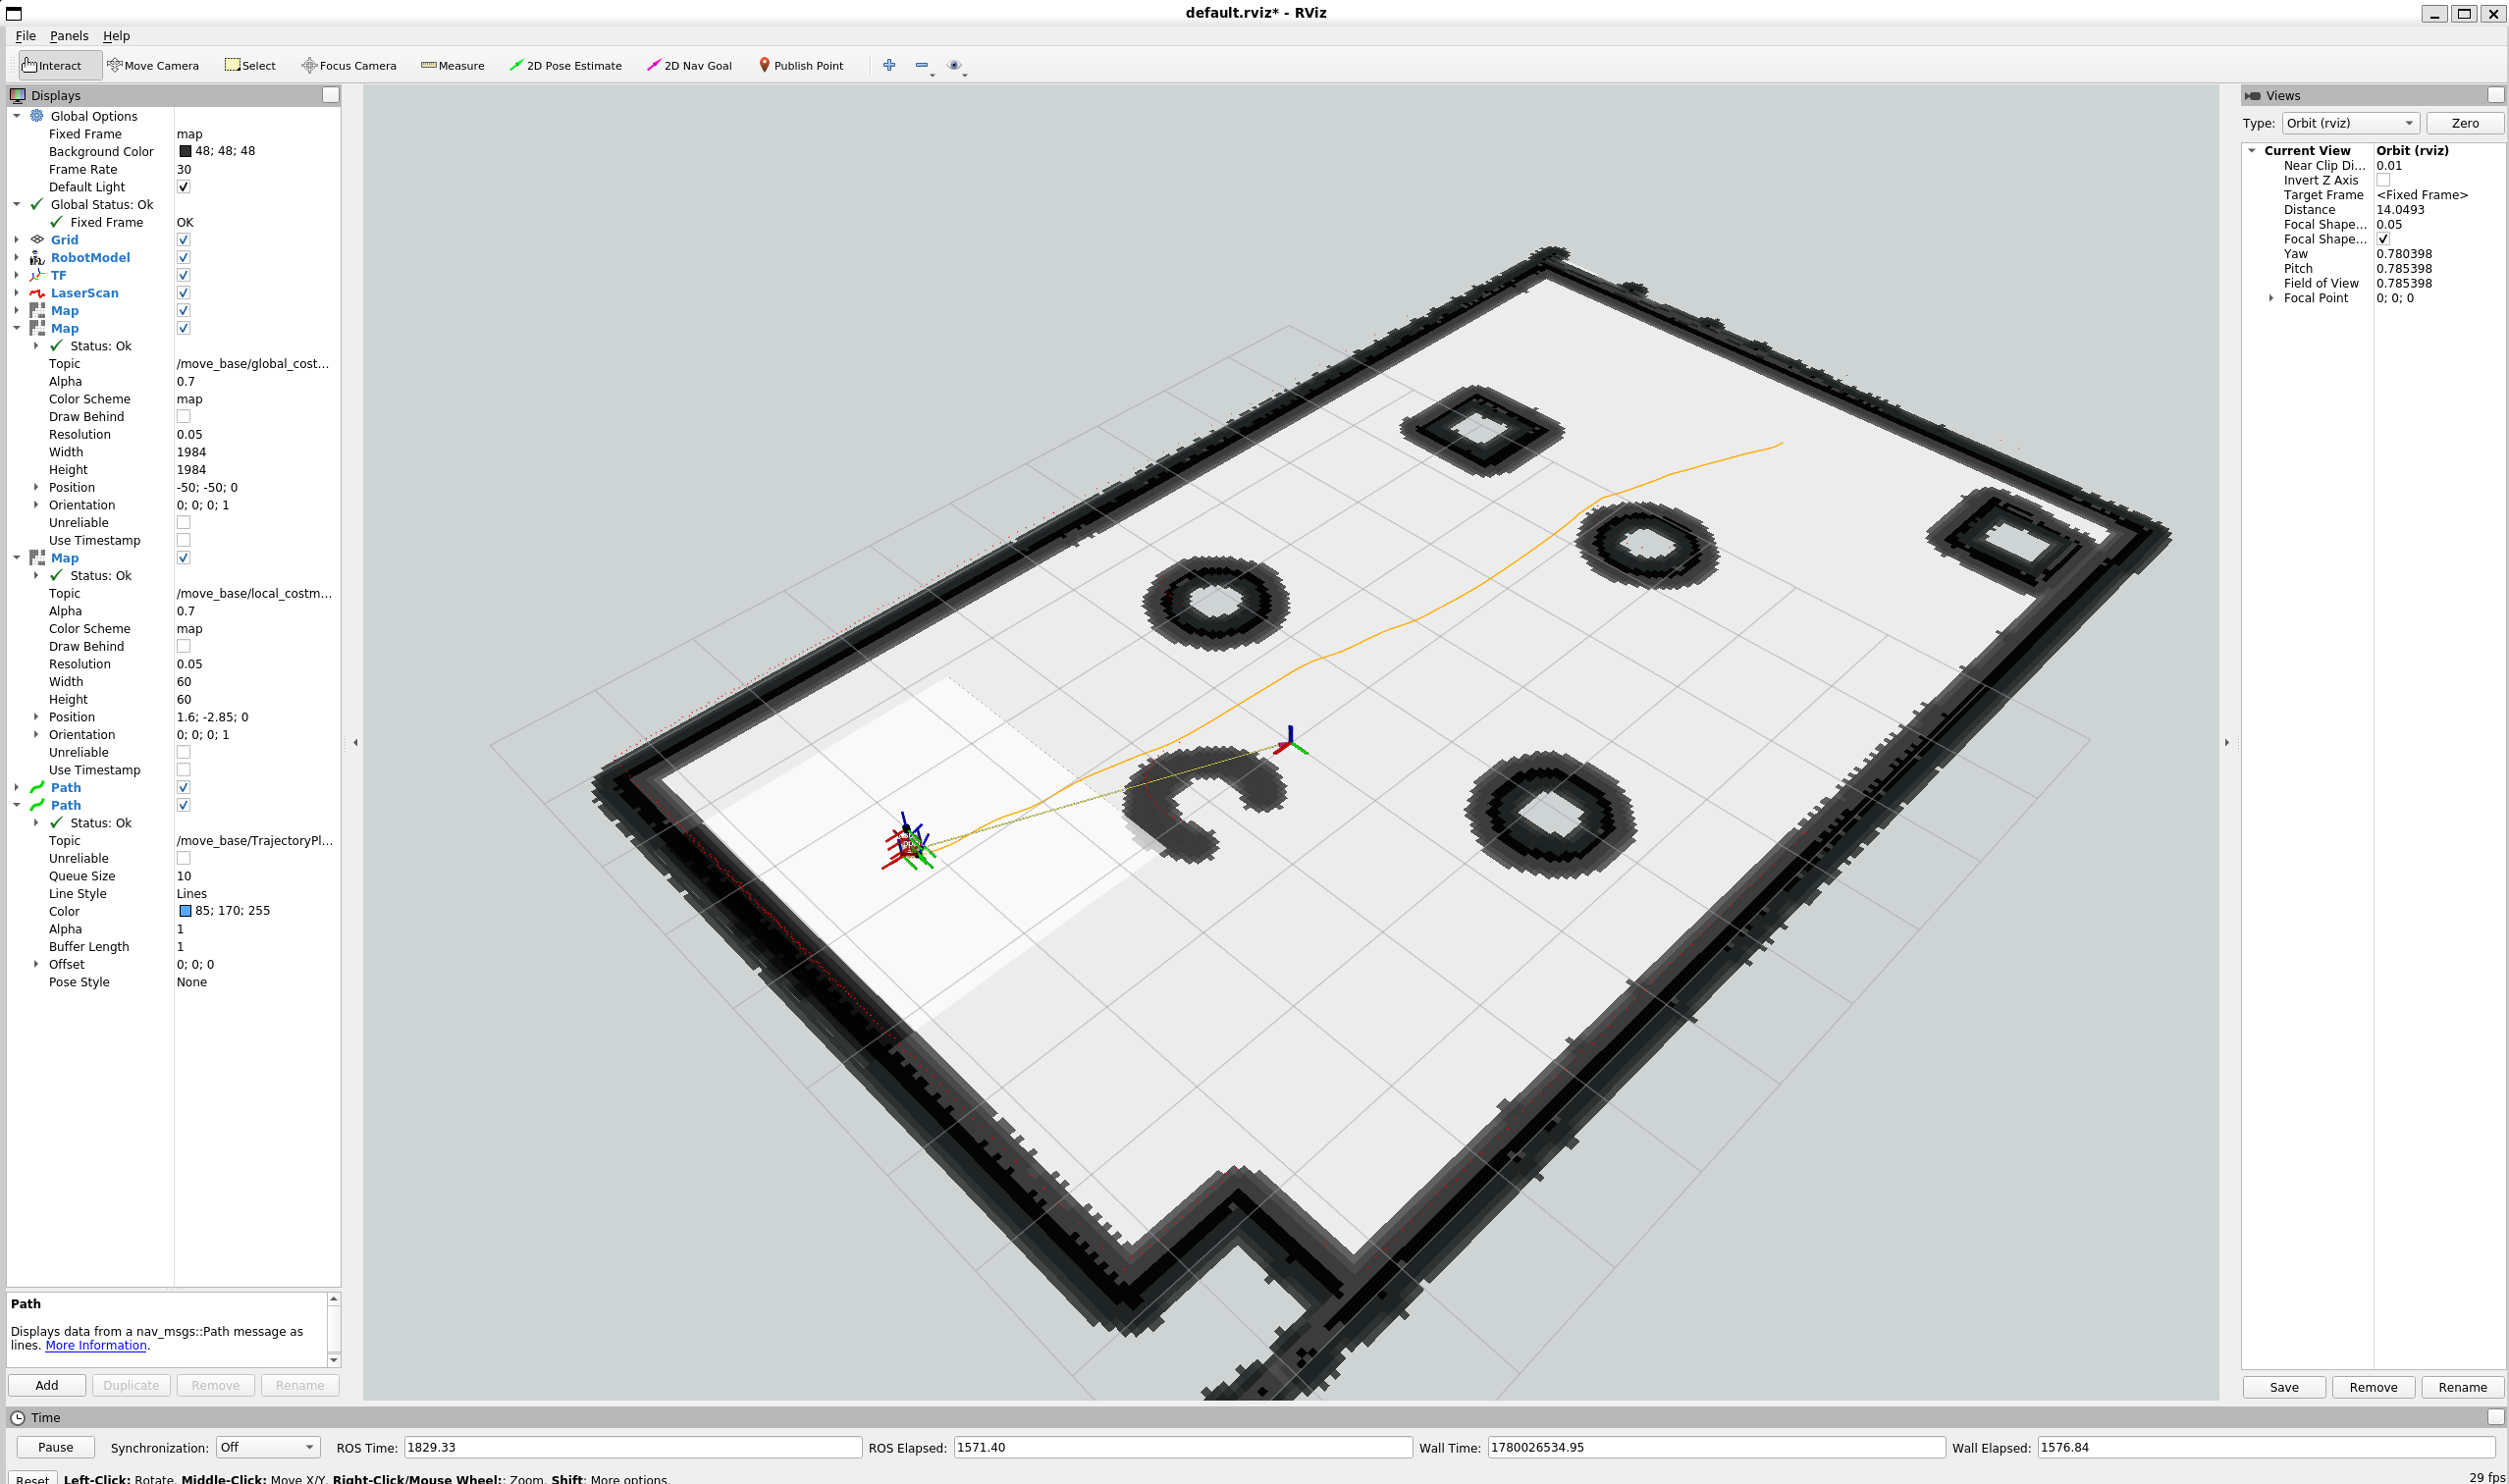
\includegraphics[width=\linewidth]{local_costmap.png}
    \caption{新增障碍物被局部代价地图实时标记并膨胀}
  \end{subfigure}
  \caption{新增未知障碍物后的局部代价地图更新。}
  \label{fig:unknown-obstacle}
\end{figure}

\subsection{动态避障与重规划效果}

当新增障碍物影响原有行驶路线时，局部代价地图会把该区域标记为不可通行或高代价区域，局部规划器在速度采样和轨迹评分时会降低穿越障碍区的候选轨迹得分，选择更安全的绕行轨迹。若局部绕行无法恢复到全局路径，\verb|move_base| 会重新调用全局规划器生成新的宏观路径。

实验中机器人在接近障碍物时没有继续直行，而是沿局部规划曲线绕过障碍区，并在绕行后继续向目标点移动。图 \ref{fig:dynamic-replan} 显示的是 RViz 中全局路径、局部代价地图、局部路径和机器人位姿的综合状态，验证了 \verb|obstacle_layer|、\verb|inflation_layer| 与局部规划器之间的数据闭环。

\begin{figure}[H]
  \centering
  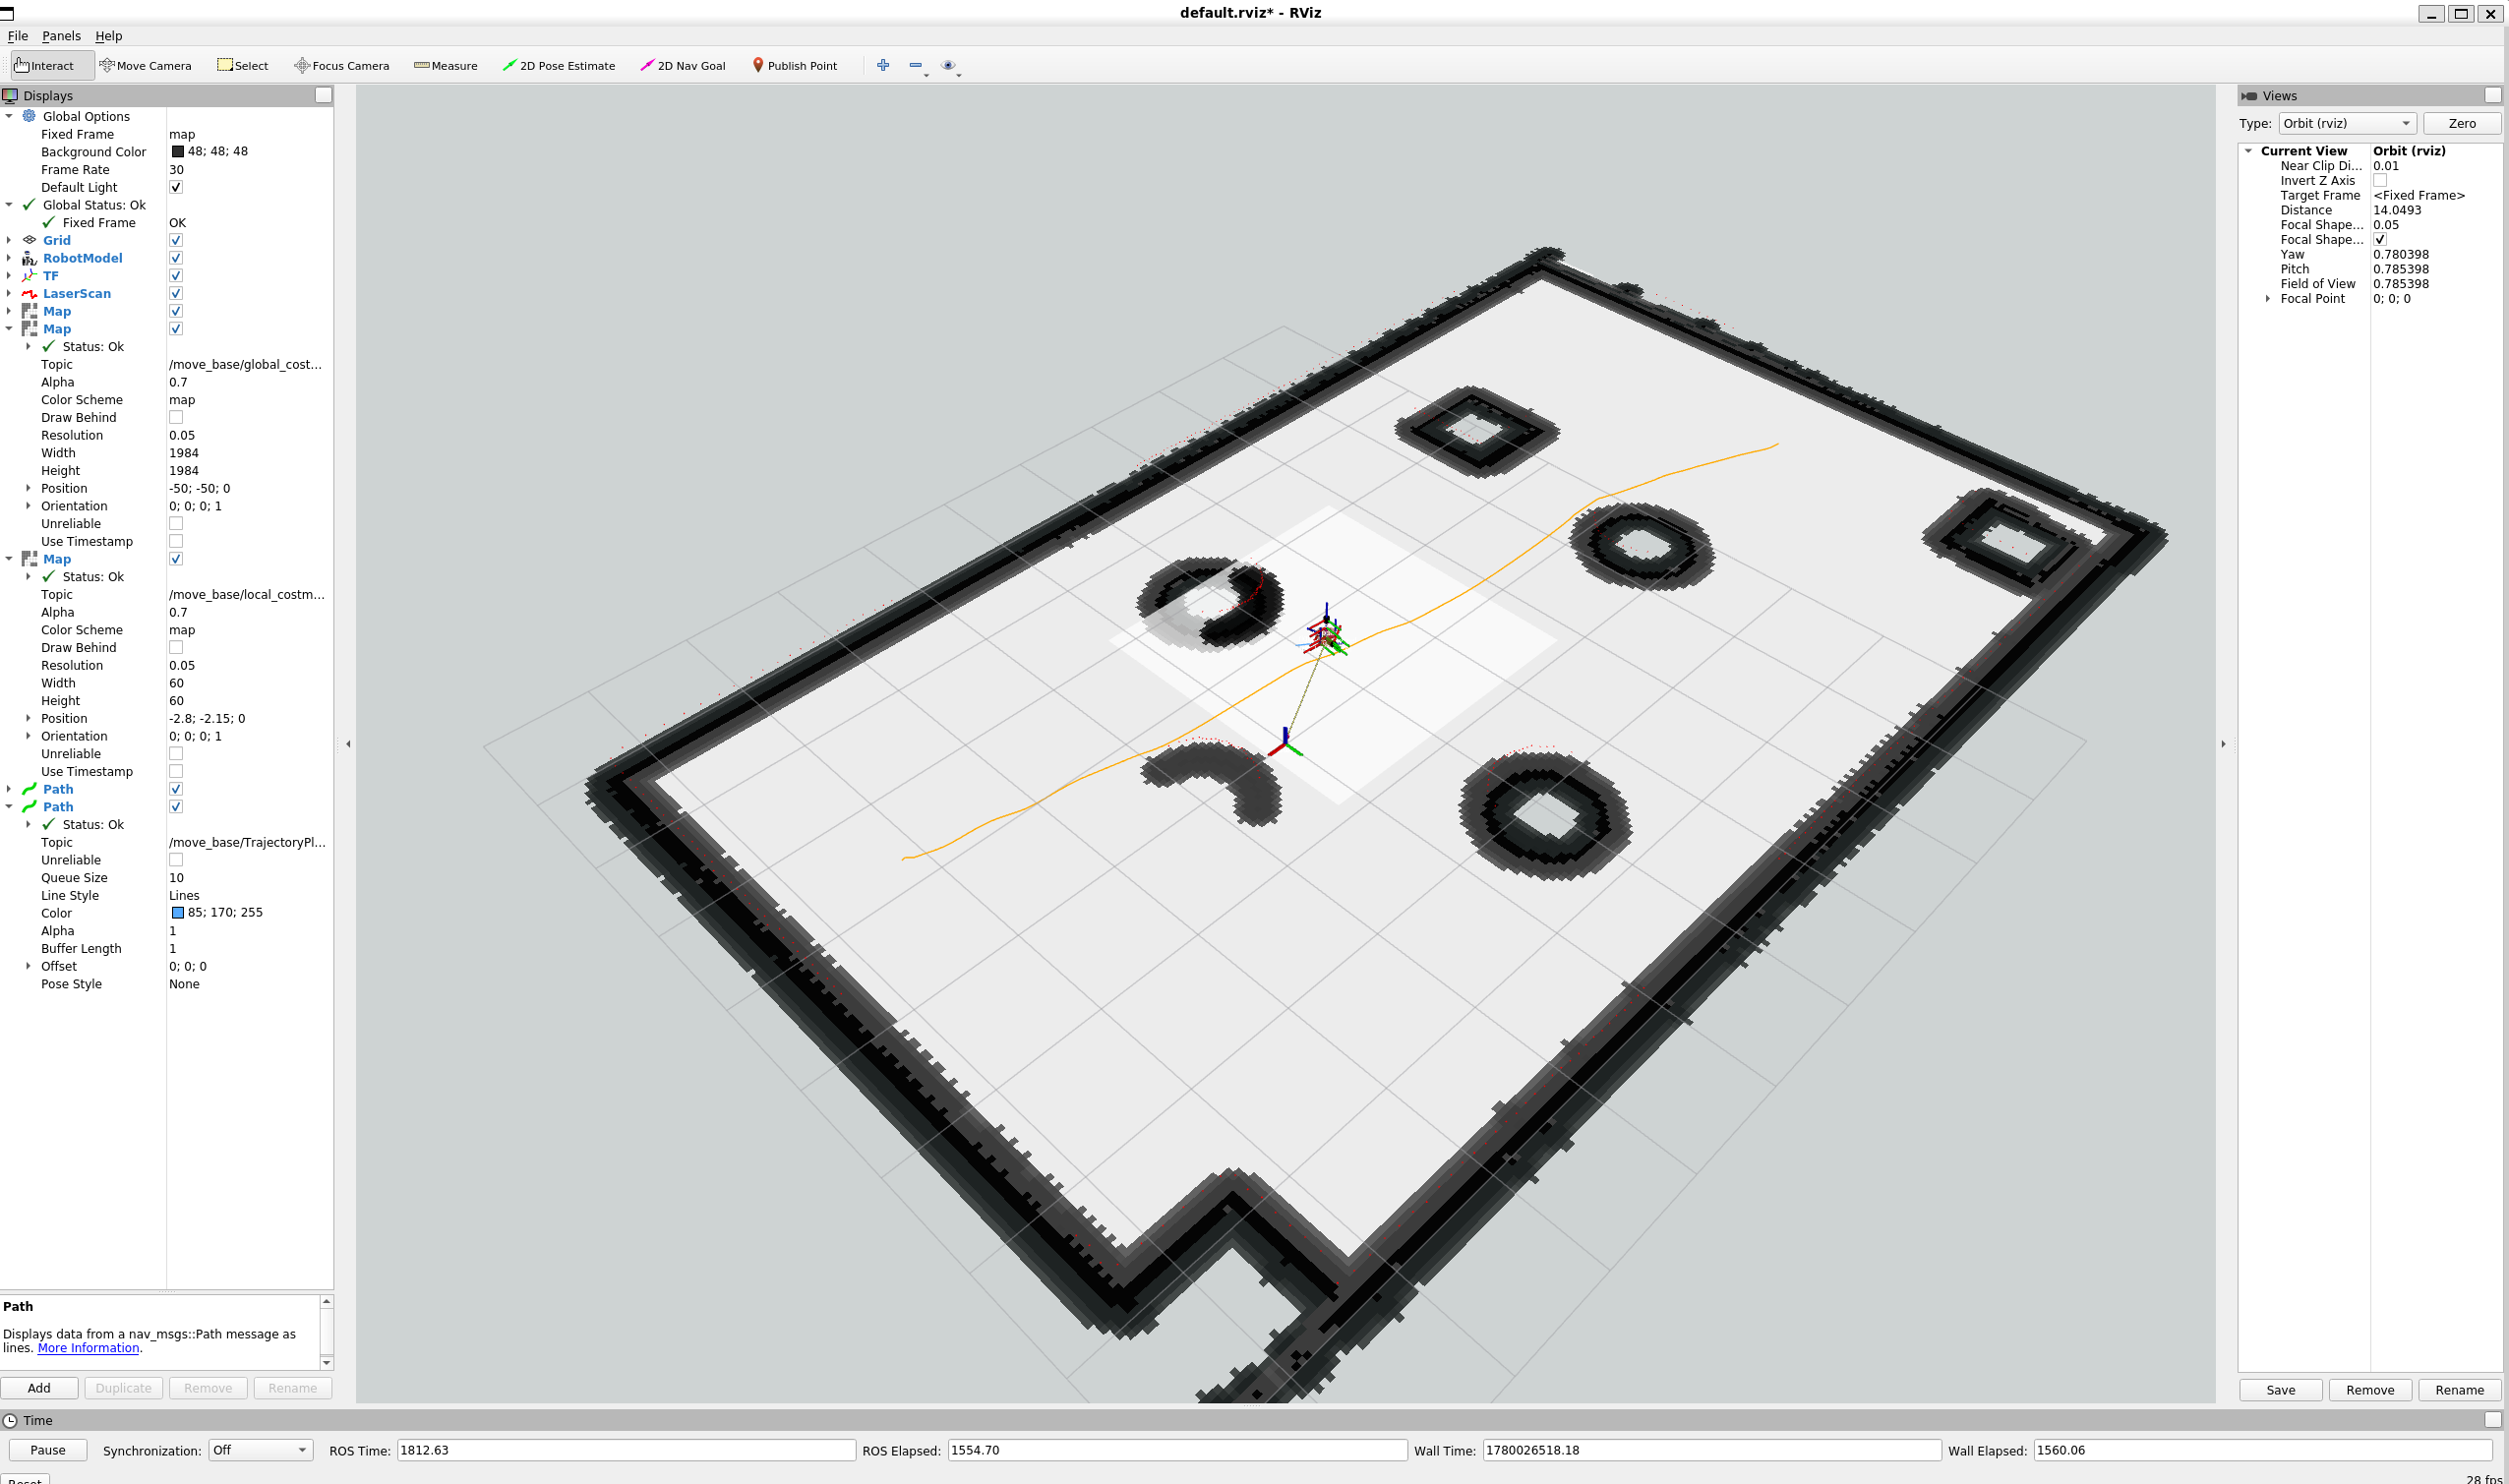
\includegraphics[width=0.92\linewidth]{dynamic_replan.png}
  \caption{RViz 中新增障碍物后的局部绕障与路径调整状态。}
  \label{fig:dynamic-replan}
\end{figure}

\section{结论}

本次实验完成了 \verb|move_base| 导航栈的搭建和验证：首先通过 \verb|map_server| 加载实验 3 保存的静态地图，通过 AMCL 在 \verb|map| 坐标系中估计机器人位姿；随后启动 \verb|move_base|，加载全局与局部代价地图、局部规划器和恢复行为参数；最后在 RViz 中使用 2D Nav Goal 发布目标点，机器人能够生成全局路径并依靠局部规划器输出速度指令完成自主导航。

动态避障实验表明，静态地图无法反映运行过程中新增的未知障碍物，而局部代价地图能够通过 \verb|/scan| 实时标记障碍物、生成膨胀区并影响局部轨迹评分，使机器人绕开临时障碍物继续前往目标点。这说明导航系统中全局代价地图和局部代价地图具有不同分工：前者保证全局路径的可达性和宏观方向，后者保证运动执行过程中的实时安全。

\section{思考题}

\textbf{通过 RViz 工具栏中 2D Nav Goal 按钮发布的目标点坐标，对应导航框架中哪个话题？目标点坐标还有其他发布方式吗？}

RViz 工具栏中的 2D Nav Goal 会把目标位姿发布到 \verb|/move_base_simple/goal|，消息类型为 \verb|geometry_msgs/PoseStamped|。除 RViz 外，还可以使用 \verb|rostopic pub| 直接向该话题发布目标点，也可以编写 \verb|actionlib| 客户端向 \verb|/move_base| Action 服务器发送 \verb|move_base_msgs/MoveBaseGoal|。后者可以获得执行中、成功、失败等状态反馈，更适合程序化导航任务。

\textbf{全局路径规划与局部路径规划的区别有哪些？}

全局路径规划面向整张静态地图或全局代价地图，主要解决从起点到终点的大方向和宏观最优路径问题，输出通常是 \verb|nav_msgs/Path|；局部路径规划面向机器人附近的小范围窗口，结合实时传感器数据和机器人运动学约束，输出下一时刻的速度指令 \verb|/cmd_vel|。全局规划更新频率较低，关注可达性和路径长度；局部规划更新频率较高，关注实时避障、轨迹平滑和运动安全。

\textbf{为什么导航系统需要同时维护“全局代价地图”和“局部代价地图”？两张地图的作用分别是什么？}

全局代价地图覆盖范围大，通常以 \verb|map| 为全局坐标系，并加载静态地图层，适合全局规划器计算从当前位置到目标点的宏观路线。局部代价地图覆盖范围小，通常以 \verb|odom| 为参考坐标系，并采用 \verb|rolling_window| 跟随机器人移动，适合快速融合激光雷达等传感器数据，处理新增障碍物和局部避障。若只使用全局代价地图，实时性和动态避障能力不足；若只使用局部代价地图，机器人容易失去整体方向，难以规划长距离可达路径。

\textbf{请给出 Action 通信与 Topic、Service 通信的区别。}

Topic 是异步发布订阅通信，适合连续数据流，例如 \verb|/scan|、\verb|/cmd_vel| 和 \verb|/odom|；Service 是同步请求-响应通信，适合一次性、短时完成的查询或控制；Action 面向长时间运行且需要状态反馈的任务，包含 goal、feedback、result 和 cancel 等机制。导航目标属于典型 Action 场景，因为机器人从当前位置移动到目标点需要持续执行、反馈过程状态，并允许中途取消或重新发送目标。

\end{document}
